\section{Date: 2026-11-13}
\noindent \textbf{Series ID: CIS2023211000000I} 

\noindent This series is titled Employment Cost Index: Wages and salaries for Private industry workers in Aircraft manufacturing and has a frequency of Quarterly. The units are Index Dec 2005=100 and the seasonal adjustment is Seasonally Adjusted.The observation start date is 2003-01-01 and the observation end date is 2026-07-01.The popularity of this series is 17. \\ 

\noindent \textbf{Series ID: FORLTAGCYVALCHG13056} 

\noindent This series is titled Valuation Change on Foreign Portfolio Holdings of U.S. Long-Term Agency Bonds: Channel Islands and Isle of Man (DISCONTINUED) and has a frequency of Monthly. The units are Millions of Dollars and the seasonal adjustment is Not Seasonally Adjusted.The observation start date is 2000-04-01 and the observation end date is 2011-12-01.The popularity of this series is 1. \\ 

\subsection{Raw Regression}
\noindent Regresses the two series against each other directly. A significant result here can come just as easily from both series sharing a long-run trend as from any real relationship.

\begin{center}
\begin{tabular}{lclc}
\toprule
\textbf{Dep. Variable:}                 & value\_fred\_FORLTAGCYVALCHG13056 & \textbf{  R-squared:         } &     0.227   \\
\textbf{Model:}                         &                OLS                & \textbf{  Adj. R-squared:    } &     0.204   \\
\textbf{Method:}                        &           Least Squares           & \textbf{  F-statistic:       } &     9.994   \\
\textbf{Date:}                          &          Fri, 13 Nov 2026         & \textbf{  Prob (F-statistic):} &  0.00330    \\
\textbf{Time:}                          &              18:57:24             & \textbf{  Log-Likelihood:    } &   -162.35   \\
\textbf{No. Observations:}              &                   36              & \textbf{  AIC:               } &     328.7   \\
\textbf{Df Residuals:}                  &                   34              & \textbf{  BIC:               } &     331.9   \\
\textbf{Df Model:}                      &                    1              & \textbf{                     } &             \\
\textbf{Covariance Type:}               &             nonrobust             & \textbf{                     } &             \\
\bottomrule
\end{tabular}
\begin{tabular}{lcccccc}
                                        & \textbf{coef} & \textbf{std err} & \textbf{t} & \textbf{P$> |$t$|$} & \textbf{[0.025} & \textbf{0.975]}  \\
\midrule
\textbf{const}                          &    -172.8673  &       53.085     &    -3.256  &         0.003        &     -280.750    &      -64.985     \\
\textbf{value\_fred\_CIS2023211000000I} &       1.5915  &        0.503     &     3.161  &         0.003        &        0.568    &        2.615     \\
\bottomrule
\end{tabular}
\begin{tabular}{lclc}
\textbf{Omnibus:}       &  1.315 & \textbf{  Durbin-Watson:     } &    2.400  \\
\textbf{Prob(Omnibus):} &  0.518 & \textbf{  Jarque-Bera (JB):  } &    0.856  \\
\textbf{Skew:}          & -0.378 & \textbf{  Prob(JB):          } &    0.652  \\
\textbf{Kurtosis:}      &  3.000 & \textbf{  Cond. No.          } & 1.48e+03  \\
\bottomrule
\end{tabular}
%\caption{OLS Regression Results}
\end{center}

Notes: \newline
 [1] Standard Errors assume that the covariance matrix of the errors is correctly specified. \newline
 [2] The condition number is large, 1.48e+03. This might indicate that there are \newline
 strong multicollinearity or other numerical problems.

\begin{figure}
\centering
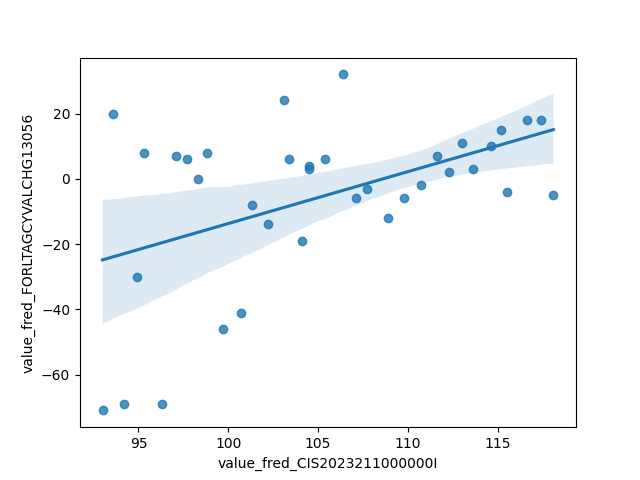
\includegraphics[scale = 0.9]{plots/plot_2026-11-13.png}
\caption{Raw Regression Plot for 2026-11-13}
\end{figure}
\newpage
\subsection{Detrended Regression}
\noindent Regresses the residuals of each series after removing its own linear time trend, so a shared trend can no longer drive the result on its own. A relationship that stays significant here is better evidence of a genuine link between the two series.

\begin{center}
\begin{tabular}{lclc}
\toprule
\textbf{Dep. Variable:}                            & value\_fred\_FORLTAGCYVALCHG13056\_detrended & \textbf{  R-squared:         } &     0.025   \\
\textbf{Model:}                                    &                     OLS                      & \textbf{  Adj. R-squared:    } &    -0.003   \\
\textbf{Method:}                                   &                Least Squares                 & \textbf{  F-statistic:       } &    0.8848   \\
\textbf{Date:}                                     &               Fri, 13 Nov 2026               & \textbf{  Prob (F-statistic):} &    0.354    \\
\textbf{Time:}                                     &                   18:57:24                   & \textbf{  Log-Likelihood:    } &   -161.73   \\
\textbf{No. Observations:}                         &                        36                    & \textbf{  AIC:               } &     327.5   \\
\textbf{Df Residuals:}                             &                        34                    & \textbf{  BIC:               } &     330.6   \\
\textbf{Df Model:}                                 &                         1                    & \textbf{                     } &             \\
\textbf{Covariance Type:}                          &                  nonrobust                   & \textbf{                     } &             \\
\bottomrule
\end{tabular}
\begin{tabular}{lcccccc}
                                                   & \textbf{coef} & \textbf{std err} & \textbf{t} & \textbf{P$> |$t$|$} & \textbf{[0.025} & \textbf{0.975]}  \\
\midrule
\textbf{const}                                     &    2.928e-11  &        3.707     &   7.9e-12  &         1.000        &       -7.534    &        7.534     \\
\textbf{value\_fred\_CIS2023211000000I\_detrended} &      -9.5168  &       10.117     &    -0.941  &         0.354        &      -30.078    &       11.044     \\
\bottomrule
\end{tabular}
\begin{tabular}{lclc}
\textbf{Omnibus:}       &  0.467 & \textbf{  Durbin-Watson:     } &    2.485  \\
\textbf{Prob(Omnibus):} &  0.792 & \textbf{  Jarque-Bera (JB):  } &    0.219  \\
\textbf{Skew:}          & -0.190 & \textbf{  Prob(JB):          } &    0.896  \\
\textbf{Kurtosis:}      &  2.966 & \textbf{  Cond. No.          } &     2.73  \\
\bottomrule
\end{tabular}
%\caption{OLS Regression Results}
\end{center}

Notes: \newline
 [1] Standard Errors assume that the covariance matrix of the errors is correctly specified.

\begin{figure}
\centering
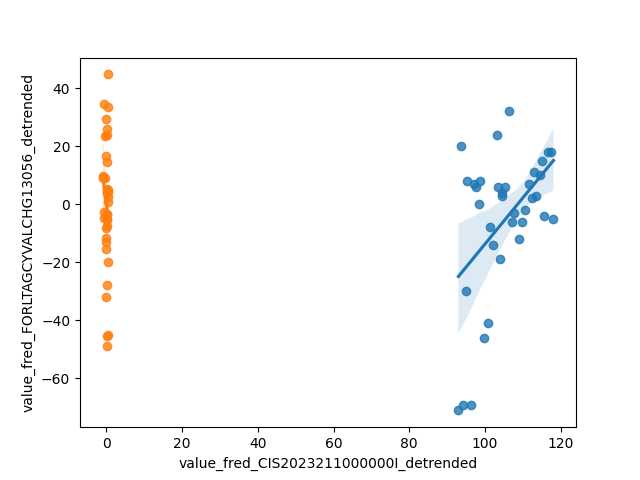
\includegraphics[scale = 0.9]{plots/plot_2026-11-13_detrended.png}
\caption{Detrended Regression Plot for 2026-11-13}
\end{figure}
\newpage
